\documentclass[3p,times,procedia]{elsarticle}
\usepackage{ecrc}
\usepackage[T1]{fontenc}
\usepackage{amsmath,amssymb,booktabs,graphicx,longtable,array}
\usepackage[bookmarks=false,colorlinks=true,linkcolor=blue,citecolor=blue,urlcolor=blue]{hyperref}
\volume{00}\firstpage{1}\journalname{Procedia Computer Science}
\runauth{Aditya Kumar et al.}\jid{procs}
\newcommand{\NC}{\textsc{NC}}
\begin{document}
\begin{frontmatter}
\title{CropXAI: Quantifying the Accuracy--Trust Gap in Earth Observation Vision Models}
\author{Aditya Kumar}\author{Govind Upadhyay}\author{Nitin Rathour}\author{Sanjay Patidar}
\address{Department of Software Engineering, Delhi Technological University, Delhi, India}
\begin{abstract}
CropXAI reports predictive, calibration, explanation, robustness, uncertainty and feature-space measures of Earth observation classifiers together with auditable run records. This revision evaluates 4 architectures on EuroSAT land-cover classification, each with 5 independent seeds and a frozen backbone: three ImageNet-pretrained models on RGB patches and the Prithvi-EO-1.0-100M encoder on six Sentinel-2 bands; the two input types are never conflated and no 13-band experiment is claimed. Test accuracy ranged from 86.31\% (Prithvi, six bands) to 96.60\% (ConvNeXt-T), while attribution stability under noise was low for all models (SSIM 0.25--0.39); explanation stability and deletion-based faithfulness are measured separately. A six-component Composite Trust Score, a weighted sum rather than a Bayesian posterior, is reported with seed-level intervals and a weight-sensitivity analysis; a post-hoc control check shows that its model ranking depends on how the explanation component is defined. An audit of the submitted results found that its Table~I pooled one- and five-epoch runs (ResNet-18: 91.53\% pooled versus 92.52\% for five-epoch runs), that fixed fallback trust values contaminated five runs, and that the model labelled Prithvi-100M was an RGB ViT-Base proxy; these results are withdrawn. The evidence covers one dataset, a random split and synthetic corruptions only, and does not validate crop-health applications.
\end{abstract}
\begin{keyword}Earth observation \sep EuroSAT \sep Prithvi \sep Explainability evaluation \sep Calibration \sep Reproducibility\end{keyword}
\end{frontmatter}

\noindent\textbf{Revision status, Paper 445.} Revised after a full re-execution of the experiments. Remaining open items are listed in the submission checklist: independent similarity report, confirmation of the conference-specific format, and the limits stated in Section~\ref{sec:limitations}.

\section{Introduction}\label{sec:introduction}
Land-cover recognition from satellite imagery is a practical setting for evaluating computer vision beyond aggregate accuracy. EuroSAT supplies labeled Sentinel-2 patches for this task \cite{eurosat}. Prediction accuracy, probability calibration and the response of explanations to perturbations describe different properties; one does not establish the others \cite{calibration,rise}. CropXAI therefore records these quantities separately and only then applies a transparent, preference-dependent summary.

The evaluated scope is \textbf{EuroSAT land-cover classification}. It does not validate crop-health diagnosis, disease detection, yield estimation or field-level stress assessment; such applications need dedicated labels and domain validation. Two input representations are evaluated and are never conflated: three ImageNet-pretrained architectures receive \emph{RGB} patches, and the geospatial foundation model Prithvi-EO-1.0-100M receives \emph{six Sentinel-2 bands}. No experiment in this paper uses all 13 Sentinel-2 bands. The retained title names the motivating question; it does not assert a universal or statistically established accuracy--trust gap.

The contribution is a tested integration of standard metrics, explicit input and checkpoint identities, and provenance-linked reporting, together with an audit of the submitted version of this work. We do not propose a new Bayesian inference method or claim that existing geospatial frameworks lack reproducibility support.

\section{Related work and comparison}\label{sec:related}
EuroSAT provides a land-use and land-cover benchmark \cite{eurosat}. ResNet \cite{resnet}, ViT \cite{vit} and ConvNeXt \cite{convnext} offer distinct visual feature extractors. Prithvi-EO-1.0 is a masked-autoencoder ViT pretrained on Harmonized Landsat Sentinel-2 (HLS) surface reflectance in six bands and three time steps \cite{prithvi,prithvicard,hls,mae}. Because its inputs differ from those of the RGB models, our comparison with it is explicitly confounded (Section~\ref{sec:models}).

Calibration analysis \cite{calibration}, attribution analysis \cite{attribution,gradcam}, perturbation-based explanation evaluation \cite{rise}, and corruption benchmarking \cite{corruptions} motivate complementary measurements. TorchGeo already provides geospatial datasets, samplers and benchmark tooling \cite{torchgeo}. CropXAI's narrower contribution is to connect such evaluations with traceable records and consistent publication assets.

\begin{center}\small
\textbf{Methodological literature comparison.} Published scores are not pooled with controlled CropXAI runs.\par\medskip
\begin{tabular}{p{.23\linewidth}p{.29\linewidth}p{.39\linewidth}}\toprule
Work & Evaluation focus & Relationship and comparison limit\\\midrule
Helber et al. \cite{eurosat} & EuroSAT classification benchmarks & Dataset and baseline context; original training/splits differ.\\
Jakubik et al. \cite{prithvi} & HLS foundation-model tasks & Spectral/temporal pretraining; our frozen linear probe on EuroSAT is not their fine-tuning protocol.\\
Guo et al. \cite{calibration} & Probability calibration & ECE motivation; temperature scaling is not evaluated here.\\
Petsiuk et al. \cite{rise} & Deletion/insertion evaluation & Deletion protocol inspiration; our attribution is not RISE.\\
Hendrycks and Dietterich \cite{corruptions} & Corruption robustness & Our two corruption families do not reproduce ImageNet-C.\\
Stewart et al. \cite{torchgeo} & Geospatial data and benchmarks & Complementary tooling; no superiority claim.\\\bottomrule
\end{tabular}\end{center}

The comparison is methodological: each source is interpreted under its original task and protocol. Only newly recorded experiments sharing the split, evaluation sample IDs and training settings can form a controlled comparison; inputs and pretraining still differ between the RGB and six-band cohorts. Different pretraining histories and feature dimensions remain limitations. The repository includes a fuller comparison matrix with source URLs, datasets, metrics and protocol differences.

\section{Implementation and evaluation protocol}\label{sec:implementation}
The validated workflow consists of dataset validation, an explicit model registry, frozen-backbone training, evaluation, immutable provenance records and result-driven reporting. Legacy research prototypes remain archived or isolated; their presence is not treated as evidence of completed experiments. Figure~\ref{fig:architecture} shows the implemented path.
\begin{figure}[htbp]\centering
\fbox{\parbox{.94\linewidth}{\centering
Hashed splits (JPEG and GeoTIFF) $\rightarrow$ checkpoint-verified model registry\\[3pt]
$\downarrow$\\[3pt]
Frozen features and seeded linear head $\rightarrow$ checkpoint/history\\[3pt]
$\downarrow$\\[3pt]
Probabilities, explanations, corruptions and embeddings\\[3pt]
$\downarrow$\\[3pt]
Metrics $\rightarrow$ immutable JSON/SQLite $\rightarrow$ tables, figures and checks}}
\caption{Implemented system architecture. Artifact hashes link generated results to individual runs.}\label{fig:architecture}
\end{figure}

\subsection{Datasets, inputs and preprocessing}\label{sec:data}
The local EuroSAT copy contains 27,000 patches of 64$\times$64 pixels in ten classes. The preserved class-wise random split has 18,900 training, 4,050 validation and 4,050 test patches; classes hold 2,000, 2,500 or 3,000 patches, so the distribution is not balanced. Content hashes found no identical file or decoded-pixel pair across splits, which does not exclude spatial proximity, near-duplicates or label errors. The split is random within classes and \emph{not} geographically independent. The upstream release version is not recorded locally; content-hashed manifests identify the exact files.

\textbf{RGB representation.} The 27,000 JPEG files (three channels, Sentinel-2 B04/B03/B02 after the provider's unspecified contrast stretch \cite{eurosat}) are resized to 224$\times$224 (bilinear, antialiased), scaled to $[0,1]$ and normalized with ImageNet statistics. Training alone uses a horizontal flip.

\textbf{Six-band representation.} The 13-band Sentinel-2 GeoTIFFs (uint16) were paired with the JPEG split by file stem; channel-mean correlation between paired JPEG and GeoTIFF red, green and blue is $\ge$ 0.999 over 200 sampled patches. The files carry no band metadata, and their storage order differs from the nominal listing: B8A is stored last. We inferred the order from spectral physics and enforce it by assertions (B8A correlates 0.98 with B08 but B09 only 0.75; B10 cirrus has a mean of 12 DN; B11 exceeds B12). The six bands passed to Prithvi are B02, B03, B04, B8A, B11 and B12 (GeoTIFF indices 1, 2, 3, 12, 10, 11), bilinearly upsampled to 224$\times$224 and standardized with Prithvi's own pretraining statistics; no statistic is fitted on evaluation data.

\subsection{Models and training}\label{sec:models}
The RGB cohort uses ResNet-18, ViT-Base/16 and ConvNeXt-T with locally cached torchvision ImageNet-1K V1 weights \cite{resnet,vit,convnext}; file hashes are verified at load. The six-band cohort uses the encoder of Prithvi-EO-1.0-100M (Hugging Face revision \texttt{f3a9ea7a}, SHA-256 \texttt{7fac0c8a...}) \cite{prithvi,prithvicard}. \textbf{Band adaptation:} Prithvi's six pretrained input channels (HLS names B02--B07: blue, green, red, narrow NIR, SWIR1, SWIR2) receive the corresponding Sentinel-2 bands; no input parameter is added or re-initialized. The pretrained network takes three time steps; one acquisition is supplied ($T{=}1$) and the three-dimensional sine--cosine position table is rebuilt for one frame and verified to equal the first-frame rows of the checkpoint table. Uncorrected differences are the processing level of the EuroSAT products (apparently Level-1C top-of-atmosphere rather than surface reflectance: the cirrus band B10, which Level-2A products omit, is present; the dataset paper does not state the level), the 64-to-224 pixel upsampling, and the absence of HLS bandpass and BRDF harmonization \cite{hls}. The classification head is linear on the mean of final-layer patch tokens \cite{mae}.

\textbf{The cohorts do not use the same bands.} RGB models see three channels; Prithvi sees six. Both share the split and the 4,050 test patches, but differ in input information, pretraining data, feature dimension and corruption units. A controlled common-input comparison is not possible without an unvalidated input adapter, so cross-cohort contrasts are descriptive and confounded.

For all models the classifier is a new ten-class linear head; backbone weights, normalization buffers and dropout are fixed (evaluation mode). Adam optimizes the head at learning rate $10^{-3}$, batch size 32, for five epochs, with seeds 42, 100, 999, 1234 and 2026. The final epoch is selected in advance; validation is diagnostic. Because the backbone is fixed, original and flipped training features are cached; cache identity includes samples, split, checkpoint hash, preprocessing and code hashes. This protocol is a new, controlled design, not an exact reconstruction of the historical trainer, which updated normalization buffers.

The submitted version mapped the name ``Prithvi-100M'' to an RGB ViT-Base proxy (Section~\ref{sec:discrepancy}); those results are withdrawn as Prithvi evidence, and unregistered model names now raise errors.

\subsection{Prediction and probability metrics}\label{sec:metrics}
In text and tables, \NC{} marks a quantity that was not computed.
Let $N$ be the number of evaluated images, $C$ the class count, $p_{ic}$ a predicted probability, $y_i$ the true class and $\hat y_i=\arg\max_c p_{ic}$. Accuracy is $N^{-1}\sum_i\mathbf{1}(\hat y_i=y_i)$. Per-class F1 is $2TP_c/(2TP_c+FP_c+FN_c)$, with zero for a zero denominator; macro-F1 averages equally across all declared classes. Weighted F1 uses class supports and is reported separately.

Using 15 equal-width confidence bins $B_b$, top-label expected calibration error is \cite{calibration}
\begin{equation}\mathrm{ECE}=\sum_b\frac{|B_b|}{N}|\mathrm{acc}(B_b)-\mathrm{conf}(B_b)|.\label{eq:ece}\end{equation}
Empty bins contribute nothing; confidence one belongs to the final bin. Negative log-likelihood is $-N^{-1}\sum_i\log p_{i,y_i}$ with a numerical floor $10^{-15}$. The multiclass Brier score is \cite{brier}
\begin{equation}B=\frac1N\sum_i\sum_c(p_{ic}-\mathbf{1}(y_i=c))^2.\label{eq:brier}\end{equation}
Normalized predictive entropy is $-\sum_c p_{ic}\log p_{ic}/\log C$, averaged over images. Entropy describes predictive dispersion, not calibrated uncertainty quality. Error-detection AUROC uses entropy to rank prediction errors and is \NC{} if only one outcome occurs.

\subsection{Explanation stability and faithfulness}\label{sec:explanation}
For an architecture-independent comparison, the revised attribution map sums absolute input-times-gradient contributions across channels \cite{attribution}, then scales each nonconstant map to [0,1]. It differs from the legacy Grad-CAM computation \cite{gradcam}. The target $t_i$ is the clean predicted class and remains fixed in every perturbed evaluation. Ten test images per class ($K=100$ images) are selected deterministically; smoke tests use one. Constant maps fail validation rather than receiving a default score.

Stability is the mean structural similarity \cite{ssim} between clean and noise-perturbed attribution maps:
\begin{equation}S=\frac1K\sum_i\mathrm{SSIM}(A_{t_i}(x_i),A_{t_i}(\tilde x_i)).\label{eq:stability}\end{equation}
Noise has standard deviation .05 on the unit scale of the representation (RGB: pixel/255; six-band: reflectance, DN/10\,000), followed by clipping. A fixed seed and identical sample schedule are used across models. Stability does not establish faithfulness.

Deletion evaluates faithfulness to model response \cite{rise}. We rank 16$\times$16 patches by mean absolute attribution, with deterministic ties, and replace the most salient patches by normalized zero (the per-channel mean of the input statistics). At 20 deletion steps, including intact and fully masked endpoints, the fixed target probability $q_{ik}$ is recorded. With $L=20$ deletion steps (before merging identical counts), actual deleted fractions $f_0=0<\dots<f_L=1$ and $K=100$ images (the same as in Eq.~\eqref{eq:stability}),
\begin{equation}D=\frac1K\sum_i\sum_{k=1}^{L}\frac{q_{i,k-1}+q_{ik}}2(f_k-f_{k-1}).\label{eq:deletion}\end{equation}
Lower deletion AUC $D$ means faster probability removal. AOPC averages $q_{i0}-q_{ik}$ over nonzero steps and images. Random and least-salient controls use identical inputs and masking schedules. Masking can itself cause distribution shift, and low initial confidence can lower AUC; controls and original probabilities must therefore accompany interpretation. AOPC follows \cite{aopc}. Neither metric proves agronomic validity.

\subsection{Robustness, uncertainty and representation}\label{sec:pillars}
The robustness proxy $R$ averages \emph{absolute} accuracy under Gaussian noise of standard deviation .05, .1 and .2 and brightness reductions .1, .3 and .5, applied on the unit scale of each representation before re-normalization (RGB clipped to $[0,1]$; reflectance clipped at zero). Because $R$ is an absolute accuracy it partly repeats the performance component; the accuracy-retention ratio (corrupted over clean accuracy) is reported separately. The same numerical severities are not equivalent across representations. These tests are motivated by corruption benchmarking \cite{corruptions}, but real geographic and seasonal OOD robustness remains \NC{}.

Uncertainty-quality score $U=1-B/2$ measures probabilistic forecast quality; it is not an isolated estimate of epistemic uncertainty. Representation score $Q=(s+1)/2$ uses the mean silhouette $s$ \cite{silhouette} of L2-normalized penultimate embeddings on a fixed balanced subset of 20 images per class. For each image, the silhouette compares average within-class distance $a$ with the nearest other-class mean distance $b$: $(b-a)/\max(a,b)$. It is a limited class-separation proxy and may depend on embedding dimension.

\subsection{Composite Trust Score and sensitivity}\label{sec:composite}
The six components are $\mathbf{s}=(\mathrm{macroF1},1-D,1-\mathrm{ECE},R,U,Q)$. Their documented ranges are [0,1]; no transformation depends on test-set extrema. Stability is reported separately and is not silently substituted for deletion faithfulness. The Composite Trust Score is
\begin{equation}T=\sum_{j=1}^{6}w_js_j,\qquad w_j\geq0,\quad\sum_jw_j=1.\label{eq:composite}\end{equation}
This weighted sum is not a Bayesian posterior or a calibrated probability of trustworthiness. The default weights are $1/6$, reflecting the absence of a justified operational preference. Missing or invalid components reject the score. Calibration, Brier and performance are correlated; independence is not assumed.

Sensitivity compares equal weights with reliability-priority weights $(.15,.10,.25,.25,.15,.10)$, explanation-priority weights $(.15,.35,.15,.15,.10,.10)$, and 50 seeded multiplicative perturbations in [.8,1.2] renormalized to sum to one. Scores, average-tie ranks, preferred models and Spearman correlation against default ranks are recorded. Correlation is \NC{} for one-model or constant-rank cases. No weighting is claimed to be universally optimal.

\section{Results and evidence audit}\label{sec:results}
\subsection{Experimental cohorts}\label{sec:cohorts}

All analysed numbers come from 20 completed runs: 4 architectures $\times$ 5 independent seeds, five epochs each, evaluated on the same 4,050 test patches. No run of the final cohorts failed. Earlier runs from a previous source revision, one superseded dry run and the one-epoch smoke test exist in the archive but are excluded by construction. The RGB cohort (ResNet-18, ViT-Base, ConvNeXt-T) and the six-band cohort (Prithvi-EO-1.0-100M) use different inputs; tests of one cohort against the other are marked as confounded.

\subsection{Predictive performance and component scores}\label{sec:perf}

Test accuracy was ResNet-18 94.55\% (95\% seed CI [94.27, 94.84]\%, macro-F1 0.9440); ViT-Base 96.01\% (95\% seed CI [95.70, 96.33]\%, macro-F1 0.9585); ConvNeXt-T 96.60\% (95\% seed CI [96.37, 96.83]\%, macro-F1 0.9648); Prithvi (6-band) 86.31\% (95\% seed CI [86.24, 86.38]\%, macro-F1 0.8558). Table~\ref{tab:trust} lists the six normalized components and the Composite Trust Score; Table~\ref{tab:ci} gives seed-level intervals; Table~\ref{tab:metrics} lists the underlying metrics. Figures~\ref{fig:accuracy} and \ref{fig:pillars} show the same values with their intervals. Seed intervals are narrow because only the linear head is trained (Section~\ref{sec:statistics}); the representation component is computed from the frozen features and is therefore identical across seeds (zero SD by construction); bootstrap intervals over test patches are wider and are also drawn in Figure~\ref{fig:accuracy}.

\begingroup\footnotesize\setlength{\tabcolsep}{3pt}\begin{longtable}{lcccc}
\caption{Six normalized components and Composite Trust Score on the test split (mean $\pm$ sample SD over $n=5$ independent seeds; five epochs). 95\% intervals are in Table~\ref{tab:ci}.}\label{tab:trust}\\
\toprule Component & ResNet-18 & ViT-Base & ConvNeXt-T & Prithvi (6-band) \\
\midrule\endfirsthead
\toprule Component & ResNet-18 & ViT-Base & ConvNeXt-T & Prithvi (6-band) \\
\midrule\endhead
Performance (macro-F1) & 0.944 $\pm$ 0.002 & 0.958 $\pm$ 0.003 & 0.965 $\pm$ 0.002 & 0.856 $\pm$ 0.001 \\
Explanation (1 - deletion AUC) & 0.781 $\pm$ 0.008 & 0.349 $\pm$ 0.012 & 0.301 $\pm$ 0.007 & 0.648 $\pm$ 0.005 \\
Calibration (1 - ECE) & 0.983 $\pm$ 0.002 & 0.993 $\pm$ 0.001 & 0.991 $\pm$ 0.001 & 0.926 $\pm$ 0.001 \\
Robustness (corrupted accuracy) & 0.699 $\pm$ 0.003 & 0.694 $\pm$ 0.009 & 0.656 $\pm$ 0.006 & 0.466 $\pm$ 0.005 \\
Uncertainty (1 - Brier/2) & 0.958 $\pm$ 0.001 & 0.970 $\pm$ 0.001 & 0.974 $\pm$ 0.001 & 0.896 $\pm$ 0.000 \\
Representation ((silhouette+1)/2) & 0.556 $\pm$ 0.000 & 0.536 $\pm$ 0.000 & 0.548 $\pm$ 0.000 & 0.548 $\pm$ 0.000 \\
Composite Trust Score & 0.820 $\pm$ 0.001 & 0.750 $\pm$ 0.002 & 0.739 $\pm$ 0.001 & 0.723 $\pm$ 0.001 \\
\bottomrule
\end{longtable}
\endgroup

\begin{figure}[htbp]\centering
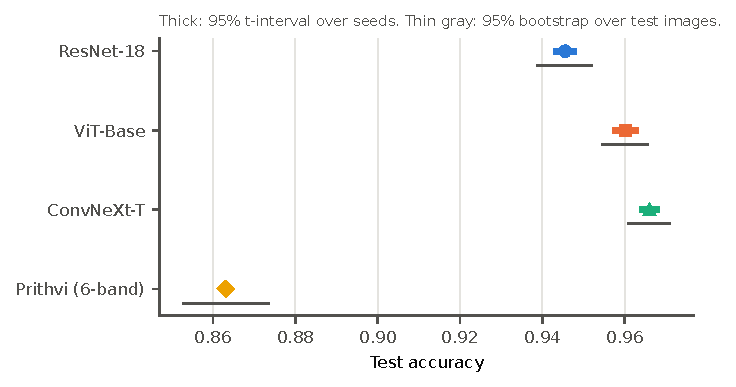
\includegraphics[width=.7\linewidth]{figures/accuracy.pdf}
\caption{Test accuracy per model. Thick bars: 95\% Student-$t$ interval over five training seeds; thin gray bars: 95\% percentile bootstrap over the 4,050 test patches (seed-averaged correctness).}\label{fig:accuracy}\end{figure}

\begin{figure}[htbp]\centering
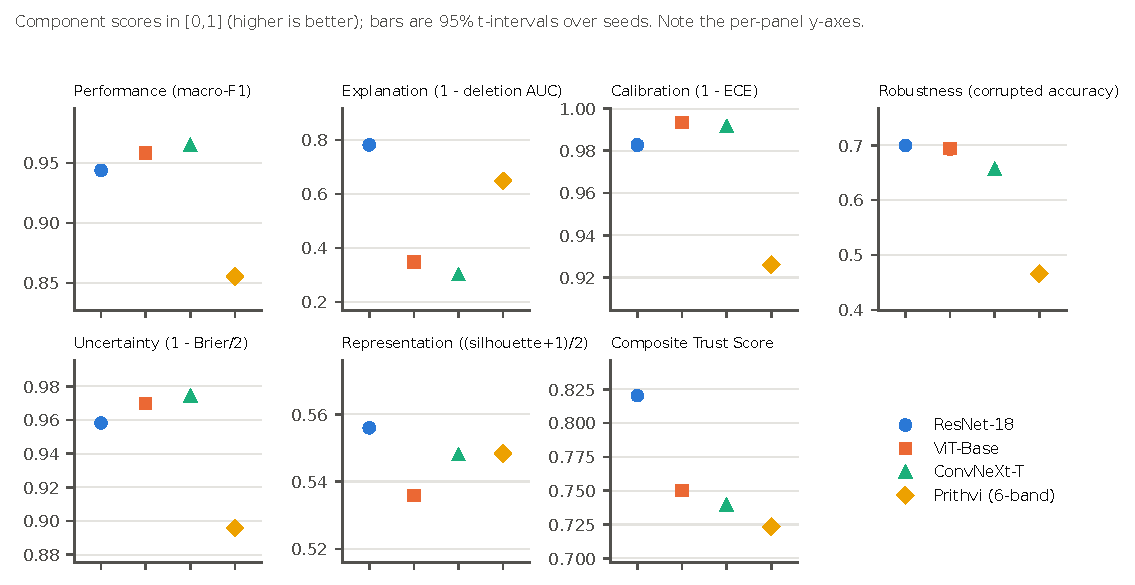
\includegraphics[width=.92\linewidth]{figures/pillars.pdf}
\caption{Six components and the Composite Trust Score (higher is better). Markers: mean over seeds; bars: 95\% Student-$t$ intervals. Each panel has its own vertical scale.}\label{fig:pillars}\end{figure}

\begingroup\scriptsize\setlength{\tabcolsep}{2pt}\begin{longtable}{lcccc}
\caption{Underlying metrics (mean $\pm$ SD over seeds). Direction: higher is better except ECE, NLL, Brier and deletion AUC of the salient order; entropy is descriptive.}\label{tab:metrics}\\
\toprule Metric & ResNet-18 & ViT-Base & ConvNeXt-T & Prithvi (6-band) \\
\midrule\endfirsthead
\toprule Metric & ResNet-18 & ViT-Base & ConvNeXt-T & Prithvi (6-band) \\
\midrule\endhead
Accuracy & 0.9455 $\pm$ 0.0023 & 0.9601 $\pm$ 0.0025 & 0.9660 $\pm$ 0.0019 & 0.8631 $\pm$ 0.0005 \\
Macro-F1 & 0.9440 $\pm$ 0.0025 & 0.9585 $\pm$ 0.0027 & 0.9648 $\pm$ 0.0021 & 0.8558 $\pm$ 0.0005 \\
ECE (15 bins) & 0.0173 $\pm$ 0.0025 & 0.0066 $\pm$ 0.0011 & 0.0085 $\pm$ 0.0006 & 0.0740 $\pm$ 0.0014 \\
NLL & 0.1652 $\pm$ 0.0040 & 0.1191 $\pm$ 0.0041 & 0.0993 $\pm$ 0.0027 & 0.4348 $\pm$ 0.0010 \\
Brier & 0.0836 $\pm$ 0.0023 & 0.0605 $\pm$ 0.0023 & 0.0515 $\pm$ 0.0016 & 0.2084 $\pm$ 0.0008 \\
Norm. entropy & 0.0944 $\pm$ 0.0009 & 0.0545 $\pm$ 0.0010 & 0.0535 $\pm$ 0.0008 & 0.2749 $\pm$ 0.0014 \\
Error-detection AUROC & 0.9098 $\pm$ 0.0025 & 0.9283 $\pm$ 0.0023 & 0.9397 $\pm$ 0.0044 & 0.8586 $\pm$ 0.0030 \\
Stability (SSIM) & 0.2473 $\pm$ 0.0014 & 0.3878 $\pm$ 0.0005 & 0.2767 $\pm$ 0.0013 & 0.3590 $\pm$ 0.0014 \\
Deletion AUC, salient & 0.2186 $\pm$ 0.0080 & 0.6510 $\pm$ 0.0118 & 0.6987 $\pm$ 0.0069 & 0.3515 $\pm$ 0.0049 \\
Deletion AUC, random & 0.1928 $\pm$ 0.0031 & 0.7165 $\pm$ 0.0094 & 0.6548 $\pm$ 0.0082 & 0.3839 $\pm$ 0.0050 \\
Deletion AUC, least salient & 0.2339 $\pm$ 0.0076 & 0.7164 $\pm$ 0.0087 & 0.7089 $\pm$ 0.0090 & 0.3997 $\pm$ 0.0045 \\
AOPC, salient & 0.7408 $\pm$ 0.0085 & 0.3438 $\pm$ 0.0120 & 0.2902 $\pm$ 0.0053 & 0.4862 $\pm$ 0.0051 \\
Silhouette & 0.1119 $\pm$ 0.0000 & 0.0718 $\pm$ 0.0000 & 0.0961 $\pm$ 0.0000 & 0.0968 $\pm$ 0.0000 \\
Accuracy retention & 0.7396 $\pm$ 0.0021 & 0.7225 $\pm$ 0.0086 & 0.6791 $\pm$ 0.0058 & 0.5401 $\pm$ 0.0059 \\
\bottomrule
\end{longtable}
\endgroup

\subsection{Calibration, explanation and robustness}\label{sec:calib}

Top-label ECE ranged from 0.0066 (ViT-Base) to 0.0740 (Prithvi (6-band)); Figure~\ref{fig:reliability} shows reliability curves pooled over seeds with the same 15 bins. Explanation stability (SSIM between attribution maps of clean and noise-perturbed inputs) was low for every model (0.247--0.388), so attributions changed substantially under $\sigma{=}.05$ noise; this does not by itself say whether the predictions or the attribution method are responsible. Deletion AUC for the most-salient-first order is compared in Figure~\ref{fig:deletion} with random and least-salient controls. The control-minus-salient AUC gap is positive when deleting salient patches removes probability faster than random deletion and negative when random deletion removes it faster (a negative gap means the attribution ranking is not more faithful than chance under this metric): ResNet-18 -0.026, ViT-Base +0.065, ConvNeXt-T -0.044, Prithvi (6-band) +0.032. Under synthetic corruption (Figure~\ref{fig:robustness}, Table~\ref{tab:corruption}) accuracy at noise $\sigma{=}.05$ ranged 0.346--0.767 and at brightness reduction $.5$ 0.476--0.951, against clean accuracies of 0.863--0.966; models differ markedly in which corruption family hurts them. These are synthetic covariate shifts on different unit scales, not geographic or seasonal shift.

\begin{figure}[htbp]\centering
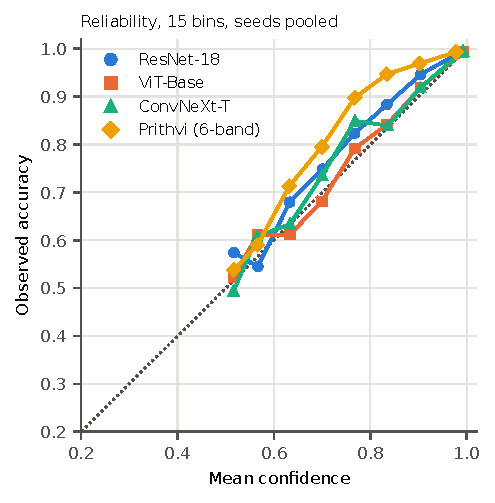
\includegraphics[width=.55\linewidth]{figures/reliability.pdf}
\caption{Reliability diagram (15 equal-width bins) with all seeds pooled per model. Dotted line: perfect calibration. Pooled values differ slightly from the per-seed mean ECE in Table~\ref{tab:metrics}.}\label{fig:reliability}\end{figure}

\begin{figure}[htbp]\centering
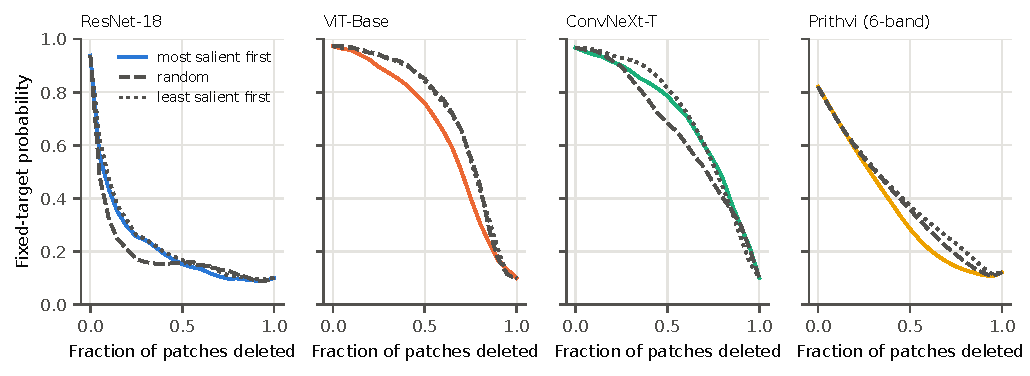
\includegraphics[width=.92\linewidth]{figures/deletion.pdf}
\caption{Fixed-target probability versus fraction of 16$\times$16 patches deleted (replacement by normalized zero), mean over 100 images and five seeds. Solid: most salient first; dashed: random; dotted: least salient first.}\label{fig:deletion}\end{figure}

\begin{figure}[htbp]\centering
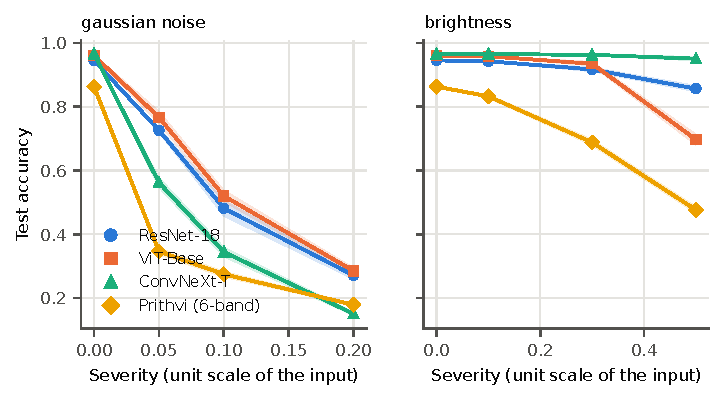
\includegraphics[width=.8\linewidth]{figures/robustness.pdf}
\caption{Test accuracy under synthetic corruptions (severity 0 is the clean test set; bands: 95\% seed intervals). Severities are on the unit scale of each input representation and are not equivalent between RGB and six-band inputs.}\label{fig:robustness}\end{figure}

\begingroup\footnotesize\setlength{\tabcolsep}{3pt}\begin{longtable}{lcccc}
\caption{Mean test accuracy under synthetic corruptions (severity in the unit scale of each input representation, so Prithvi and RGB severities are not equivalent).}\label{tab:corruption}\\
\toprule Condition & ResNet-18 & ViT-Base & ConvNeXt-T & Prithvi (6-band) \\
\midrule\endfirsthead
\toprule Condition & ResNet-18 & ViT-Base & ConvNeXt-T & Prithvi (6-band) \\
\midrule\endhead
gaussian noise 0.05 & 0.726 & 0.767 & 0.562 & 0.346 \\
gaussian noise 0.1 & 0.482 & 0.520 & 0.344 & 0.274 \\
gaussian noise 0.2 & 0.271 & 0.285 & 0.150 & 0.179 \\
brightness 0.1 & 0.943 & 0.958 & 0.965 & 0.833 \\
brightness 0.3 & 0.917 & 0.935 & 0.963 & 0.688 \\
brightness 0.5 & 0.857 & 0.697 & 0.951 & 0.476 \\
clean & 0.946 & 0.960 & 0.966 & 0.863 \\
\bottomrule
\end{longtable}
\endgroup

\subsection{Composite Trust Score, weights and ranking}\label{sec:sensresults}

Under the default (equal) weights the Composite Trust Score ranks the models as ResNet-18 > ViT-Base > ConvNeXt-T > Prithvi (6-band). Equal weights prefer ResNet-18; reliability weights prefer ResNet-18; explanation priority weights prefer ResNet-18. Across 54 weight configurations (equal, two priority profiles and 50 random perturbations of $\pm20\%$) the ranking differed from the default in 2 configuration(s); Spearman correlation with the default ranking ranged 0.40--1.00. This analysis includes models with different inputs and is therefore descriptive only (Figure~\ref{fig:sensitivity}). The weight profiles were fixed in the versioned configuration before the final campaign was executed and are a utility choice, not an estimate.

\begin{figure}[htbp]\centering
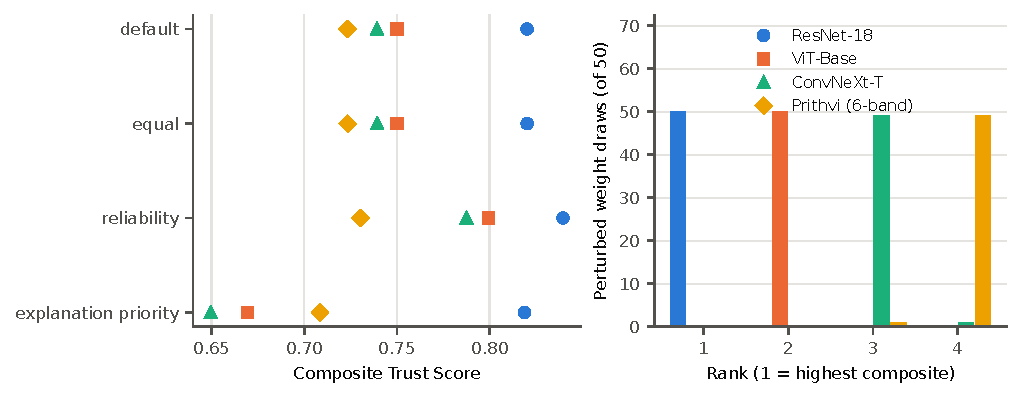
\includegraphics[width=.92\linewidth]{figures/sensitivity.pdf}
\caption{Left: Composite Trust Score under the named weight profiles. Right: how often each model attains each rank over 50 seeded random weight perturbations.}\label{fig:sensitivity}\end{figure}

\subsection{Post-hoc check of the explanation component}\label{sec:posthoc}

\textbf{This subsection is post-hoc: it was defined after the main results were inspected and does not replace the pre-declared composite.} The explanation component $1-D$ rewards low salient-first deletion AUC, but a model whose probability collapses under \emph{any} masking also has a low $D$. The random-order control exposes this: for some models random deletion removes probability faster than salient-first deletion, so a high $1-D$ then reflects fragility to masking rather than a faithful attribution. As a diagnostic only, the explanation component is replaced by $E'=\tfrac12\bigl(1+(D_{\mathrm{rand}}-D)/(D_{\mathrm{rand}}+D)\bigr)$, where $E'=.5$ means salient deletion is no faster than random deletion, $E'>.5$ faster and $E'<.5$ slower. With default weights the composite ranking changes from ResNet-18 (0.820) > ViT-Base (0.750) > ConvNeXt-T (0.739) > Prithvi (6-band) (0.723) (pre-declared) to ViT-Base (0.779) > ConvNeXt-T (0.770) > ResNet-18 (0.768) > Prithvi (6-band) (0.702) (post-hoc). Only models with $E'$ above .5 show attributions that outperform random deletion under this protocol: ResNet-18 $E'=0.469$, ViT-Base $E'=0.524$, ConvNeXt-T $E'=0.484$, Prithvi (6-band) $E'=0.522$. The composite ranking is therefore not robust to how the explanation component is defined, and no ranking is claimed to be universal.

\subsection{Pairwise comparisons}\label{sec:pairs}

Of 6 pairwise accuracy comparisons, 5 have a Bonferroni-adjusted bootstrap interval that excludes zero (Table~\ref{tab:paired}, Figure~\ref{fig:paired}). Comparisons marked with an asterisk cross input representations and cannot attribute a difference to the architecture. All comparisons are exploratory, condition on one random split, and do not support claims about geographic generalization.

\begingroup\footnotesize\setlength{\tabcolsep}{3pt}\begin{longtable}{lrlrl}
\caption{Exploratory paired differences. Accuracy: percentile bootstrap over test images (Bonferroni-adjusted level, seed-averaged correctness). Composite: Student-$t$ over paired seeds. * different input representation.}\label{tab:paired}\\
\toprule A $-$ B & $\Delta$acc & Bonf. CI (items) & $\Delta T$ & 95\% CI (seeds) \\
\midrule\endfirsthead
\toprule A $-$ B & $\Delta$acc & Bonf. CI (items) & $\Delta T$ & 95\% CI (seeds) \\
\midrule\endhead
ConvNeXt-T $-$ Prithvi (6-band) * & +0.1029 & [0.0892, 0.1167] & +0.0159 & [0.0142, 0.0176] \\
ConvNeXt-T $-$ ResNet-18 & +0.0205 & [0.0125, 0.0284] & -0.0809 & [-0.0827, -0.0792] \\
ConvNeXt-T $-$ ViT-Base & +0.0059 & [-0.0006, 0.0125] & -0.0107 & [-0.0128, -0.0087] \\
Prithvi (6-band) $-$ ResNet-18 * & -0.0824 & [-0.0969, -0.0675] & -0.0968 & [-0.0993, -0.0943] \\
Prithvi (6-band) $-$ ViT-Base * & -0.0970 & [-0.1110, -0.0833] & -0.0266 & [-0.0289, -0.0244] \\
ResNet-18 $-$ ViT-Base & -0.0146 & [-0.0235, -0.0055] & +0.0702 & [0.0670, 0.0734] \\
\bottomrule
\end{longtable}
\endgroup

\begin{figure}[htbp]\centering
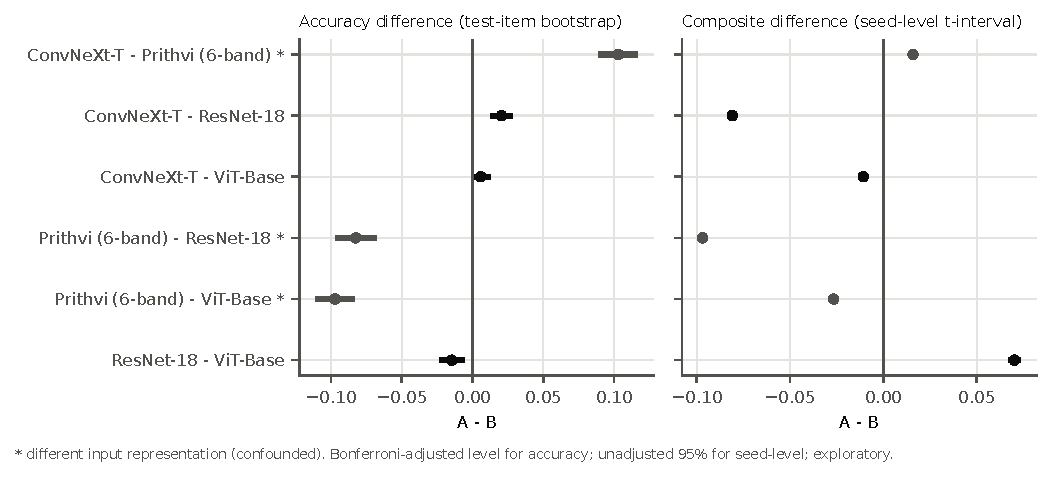
\includegraphics[width=.92\linewidth]{figures/paired_differences.pdf}
\caption{Pairwise differences (A $-$ B). Left: accuracy, bootstrap over test patches at the Bonferroni-adjusted level. Right: Composite Trust Score, 95\% Student-$t$ interval over paired seeds. Gray: different input representations.}\label{fig:paired}\end{figure}

\subsection{Training history}\label{sec:history}

Figure~\ref{fig:history} shows validation accuracy per epoch (mean $\pm$ SD over seeds) together with the final test accuracy, labelled separately. Final-epoch validation versus final test accuracy: ResNet-18 93.60\% versus 94.55\%; ViT-Base 96.19\% versus 96.01\%; ConvNeXt-T 96.40\% versus 96.60\%; Prithvi (6-band) 85.89\% versus 86.31\%. The binomial standard error of one accuracy on 4,050 patches is about 0.3--0.5 percentage points, so a one-point difference between two independent 4,050-patch subsets is within a few standard errors. Validation was never used to choose the reported epoch. Per-patch confusion matrices for one seed are in Figure~\ref{fig:confusion}.

\begin{figure}[htbp]\centering
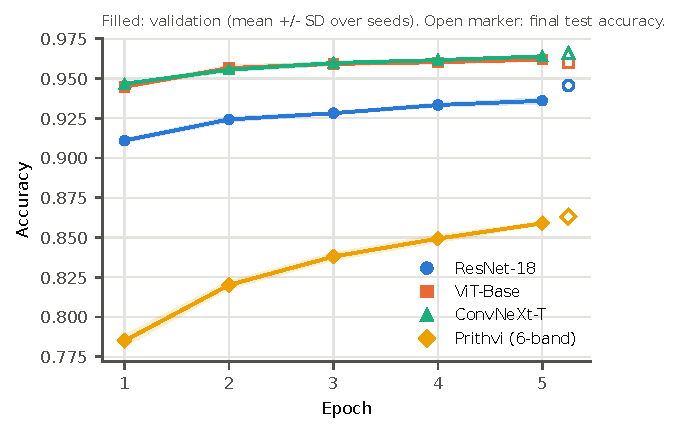
\includegraphics[width=.6\linewidth]{figures/training_history.pdf}
\caption{Validation accuracy per epoch (filled, band: $\pm$1 SD over seeds) and final test accuracy (open marker).}\label{fig:history}\end{figure}

\begin{figure}[htbp]\centering
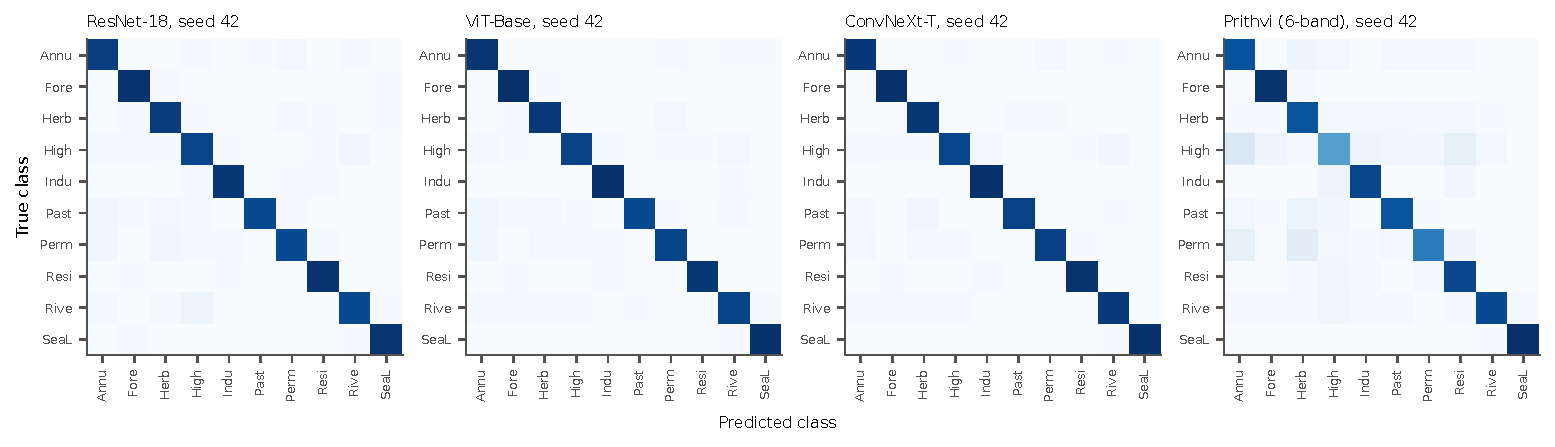
\includegraphics[width=.92\linewidth]{figures/confusion.pdf}
\caption{Row-normalized confusion matrices on the test split for the lowest seed of each model.}\label{fig:confusion}\end{figure}

\begingroup\footnotesize\setlength{\tabcolsep}{3pt}\begin{longtable}{llrrlr}
\caption{Seed-level mean, sample SD and 95\% Student-$t$ interval for every component. NC = not computed.}\label{tab:ci}\\
\toprule Model & Component & Mean & SD & 95\% CI & $n$/missing \\
\midrule\endfirsthead
\toprule Model & Component & Mean & SD & 95\% CI & $n$/missing \\
\midrule\endhead
ResNet-18 & Performance (macro-F1) & 0.9440 & 0.0025 & [0.9409, 0.9471] & 5/0 \\
ResNet-18 & Explanation (1 - deletion AUC) & 0.7814 & 0.0080 & [0.7714, 0.7914] & 5/0 \\
ResNet-18 & Calibration (1 - ECE) & 0.9827 & 0.0025 & [0.9796, 0.9858] & 5/0 \\
ResNet-18 & Robustness (corrupted accuracy) & 0.6993 & 0.0025 & [0.6962, 0.7024] & 5/0 \\
ResNet-18 & Uncertainty (1 - Brier/2) & 0.9582 & 0.0011 & [0.9568, 0.9597] & 5/0 \\
ResNet-18 & Representation ((silhouette+1)/2) & 0.5560 & 0.0000 & [0.5560, 0.5560] & 5/0 \\
ResNet-18 & Composite Trust Score & 0.8203 & 0.0009 & [0.8191, 0.8214] & 5/0 \\
ViT-Base & Performance (macro-F1) & 0.9585 & 0.0027 & [0.9552, 0.9618] & 5/0 \\
ViT-Base & Explanation (1 - deletion AUC) & 0.3490 & 0.0118 & [0.3343, 0.3636] & 5/0 \\
ViT-Base & Calibration (1 - ECE) & 0.9934 & 0.0011 & [0.9921, 0.9948] & 5/0 \\
ViT-Base & Robustness (corrupted accuracy) & 0.6938 & 0.0094 & [0.6820, 0.7055] & 5/0 \\
ViT-Base & Uncertainty (1 - Brier/2) & 0.9697 & 0.0012 & [0.9683, 0.9712] & 5/0 \\
ViT-Base & Representation ((silhouette+1)/2) & 0.5359 & 0.0000 & [0.5359, 0.5359] & 5/0 \\
ViT-Base & Composite Trust Score & 0.7500 & 0.0020 & [0.7476, 0.7525] & 5/0 \\
ConvNeXt-T & Performance (macro-F1) & 0.9648 & 0.0021 & [0.9622, 0.9674] & 5/0 \\
ConvNeXt-T & Explanation (1 - deletion AUC) & 0.3013 & 0.0069 & [0.2928, 0.3099] & 5/0 \\
ConvNeXt-T & Calibration (1 - ECE) & 0.9915 & 0.0006 & [0.9907, 0.9922] & 5/0 \\
ConvNeXt-T & Robustness (corrupted accuracy) & 0.6560 & 0.0055 & [0.6492, 0.6629] & 5/0 \\
ConvNeXt-T & Uncertainty (1 - Brier/2) & 0.9742 & 0.0008 & [0.9732, 0.9753] & 5/0 \\
ConvNeXt-T & Representation ((silhouette+1)/2) & 0.5480 & 0.0000 & [0.5480, 0.5480] & 5/0 \\
ConvNeXt-T & Composite Trust Score & 0.7393 & 0.0005 & [0.7386, 0.7400] & 5/0 \\
Prithvi (6-band) & Performance (macro-F1) & 0.8558 & 0.0005 & [0.8551, 0.8564] & 5/0 \\
Prithvi (6-band) & Explanation (1 - deletion AUC) & 0.6485 & 0.0049 & [0.6424, 0.6545] & 5/0 \\
Prithvi (6-band) & Calibration (1 - ECE) & 0.9260 & 0.0014 & [0.9243, 0.9278] & 5/0 \\
Prithvi (6-band) & Robustness (corrupted accuracy) & 0.4661 & 0.0049 & [0.4600, 0.4722] & 5/0 \\
Prithvi (6-band) & Uncertainty (1 - Brier/2) & 0.8958 & 0.0004 & [0.8953, 0.8963] & 5/0 \\
Prithvi (6-band) & Representation ((silhouette+1)/2) & 0.5484 & 0.0000 & [0.5484, 0.5484] & 5/0 \\
Prithvi (6-band) & Composite Trust Score & 0.7234 & 0.0015 & [0.7216, 0.7252] & 5/0 \\
\bottomrule
\end{longtable}
\endgroup

\subsection{Statistical analysis}\label{sec:statistics}
\textbf{Statistical unit and uncertainty.} Two sources of variation are quantified separately. (i) \emph{Training seeds}: for $n$ independent seeds under one configuration we report mean $\bar z$, sample standard deviation $s_z$ ($n-1$) and the 95\% Student-$t$ interval $\bar z\pm t_{.975,n-1}s_z/\sqrt n$; with $n<2$ these are \NC{}. Because the backbone is frozen, seeds randomize only the head initialization, batch order and flips, so seed intervals are narrow and describe optimization noise, not data variation. (ii) \emph{Test patches}: per-patch correctness averaged over seeds is resampled with a percentile bootstrap (10,000 draws, fixed seed) over the 4,050 test patches, which describes sampling noise on this fixed split. Patches, pixels and minibatches are never counted as training replicates. Neither interval reflects geographic or seasonal variance.

\textbf{Pairwise comparisons} use identical test patches; accuracy differences use the paired bootstrap at a Bonferroni-adjusted level, and seed-level differences of other metrics use paired Student-$t$ intervals over shared seeds. Seeds do not imply identical data ordering across architectures. All comparisons are exploratory. The Friedman/Nemenyi analysis and critical-difference diagram of the submitted version are withdrawn: they require many independent datasets \cite{statistics}, and seeds of one dataset are not datasets. No significance is inferred from plots.

\textbf{Sensitivity to weights} reuses the scores of Section~\ref{sec:composite}: Spearman correlation compares each scheme's ranking with the default ranking.

\section{Audit of the submitted results}\label{sec:discrepancy}
\textbf{Table I of the submitted version.} Recomputing from the stored legacy database reproduces the printed accuracies exactly as the unweighted mean over \emph{all} runs of a model, regardless of epoch count: ResNet-18 91.53\% (6 runs, of one and of five epochs), ViT-Base 95.41\% (6 runs) and ``Prithvi-100M'' 95.30\% (5 runs). Only three distinct seeds exist, not five; the five-epoch-only means are 92.52\%, 96.07\% and 96.14\%. The reported numbers therefore did not describe a five-seed, five-epoch experiment. Table~\ref{tab:legacy} compares them with the corrected cohorts.

\begin{table}[htbp]\centering\footnotesize\setlength{\tabcolsep}{3pt}\caption{Submitted accuracy versus the mixed legacy and the corrected cohorts (test accuracy, \%). Column 3: mean of legacy five-epoch runs only (number of runs). Column 4: corrected protocol, mean [95\% seed interval] over five seeds. The protocols differ (legacy trainer updated BatchNorm statistics; corrected runs train a linear head on frozen features), so the columns are not a like-for-like replication.}\label{tab:legacy}\begin{tabular}{p{.3\linewidth}rrr}\toprule Model & Submitted (1+5 epochs pooled) & Legacy, 5 epochs only & Corrected, 5 seeds $\times$ 5 epochs\\\midrule ResNet-18 & 91.53\% & 92.52 (3) & 94.55 [94.27, 94.84] \\ ViT-Base & 95.41\% & 96.07 (3) & 96.01 [95.70, 96.33] \\ ConvNeXt-T & not reported & 96.58 (3) & 96.60 [96.37, 96.83] \\ ``Prithvi-100M'' (ViT proxy) / Prithvi-EO-1.0-100M & 95.30\% & 96.14 (2), proxy & 86.31 [86.24, 86.38], real model \\\bottomrule\end{tabular}\end{table}

\textbf{Figure 7 versus Table I.} The submitted training-convergence figure (it appears as Fig.~8 in the submitted PDF, whereas its Fig.~7 is a cross-dataset drift plot; the reviewer comment calls it Figure 7) shows, for ResNet-18 over five epochs, validation accuracy of about 84--86\% and a training loss falling to about 0.50. The legacy store derives a run identifier from the configuration alone and writes metrics with \texttt{INSERT OR REPLACE}, so repeating a configuration replaced the earlier values under the unchanged run record. For the run ResNet-18, seed 42, five epochs, the reviewer-package copy of the database holds test accuracy 85.19\% and final training loss 0.499, whereas the main database, used for the submitted Table I, holds 92.37\% and 0.249 under the same identifier and timestamp. The first set agrees with the convergence figure on both quantities (accuracy band and final loss). In addition, another submitted figure file (\texttt{baseline\_results.pdf}) prints ``Final Test Accuracy: 85.19\%'' and ``Final Trust Score (T3): 0.2394'', exactly the reviewer-package values of this run and not the main-database values, and it was registered in the database about 90 seconds after the run timestamp. The second set is what entered the submitted table. We therefore conclude that the submitted figure and table come from \emph{different executions of the same configuration}, and that the figure is consistent with the original execution, not with the values later used in the table. The convergence figure's own plotted data were not preserved, so its link to that execution is strongly supported but not proven.

\textbf{Re-execution of the legacy trainer.} The unchanged legacy trainer was executed again (ResNet-18, seed 42, five epochs; the legacy database tables were verified identical to the archived original afterwards). Its validation accuracy per epoch was 89.7\%, 90.8\%, 91.9\%, 91.6\%, 92.1\%, final training loss 0.2492, test accuracy 92.37\% and weighted F1 0.9231. These reproduce the values held in the main database (92.37\%, loss 0.2492) and not the earlier reviewer-package values or the validation band of the submitted Figure 7. Hence the main-database entry is reproducible with the current legacy code (one re-execution), while the execution that produced the Figure-7-like values (accuracy 85.19\%, final loss 0.499) cannot be reproduced with the present code and data; the code revision (recorded as unknown) or data state evidently differed. Consequently the submitted figure and table describe different executions, and neither can be certified as a five-seed result.

\textbf{Fallback trust values.} The legacy trust function returned the constants 0.65 (missing library) and 0.50 (no supported layer). Five stored runs carry a trust value of exactly 0.5, including all one-epoch ``Prithvi-100M'' runs; these values are fallbacks, not measurements, and are invalid. The function now raises an error, and a test enforces this.

\textbf{The foundation-model label.} For every (epochs, seed) cell present for both, the legacy ``Prithvi-100M'' accuracy, F1, precision and recall equal those of ViT-Base to machine precision: the label denoted an RGB ViT-Base proxy. All legacy ``Prithvi-100M'' results are withdrawn; Prithvi-EO-1.0-100M is evaluated afresh in this revision. Both legacy databases and the original sources remain preserved.

\textbf{Legacy statistical code.} A scan of the legacy source tree (reproducible with a script in the repository) found modules whose own comments describe them as mock implementations, among them a Nemenyi post-hoc test, a Bayesian ranking, a power analysis, and an explanation-benchmark manager that draws deletion and insertion AUC values from a uniform random generator. The scan cannot show which of them produced numbers in the submitted manuscript; none of their output is reused here, the active pipeline contains no such code (enforced by a test), and the Nemenyi, Bayesian and power claims are withdrawn.

\section{Discussion and limitations}\label{sec:limitations}
\textbf{What the evidence supports.} Accuracy, calibration, explanation behaviour and robustness ranked the models differently, so no single number summarizes them. In particular, the most accurate RGB model (ConvNeXt-T) has the lowest pre-declared composite among the RGB models, and the composite ranking reverses under a post-hoc control normalization of the explanation component (Section~\ref{sec:posthoc}); neither ranking should be read as a statement of trustworthiness. Attribution stability under small noise was low for every model, and deletion faithfulness relative to a random-order control was mixed: two models' salient-first deletion removed probability faster than random deletion, two did not. These observations describe one attribution rule (absolute input-times-gradient), one masking baseline and one patch size.

\textbf{The Prithvi result is not a verdict on the model.} Its lower accuracy and calibration may reflect any of the following, which this experiment does not separate: a frozen encoder with a linear head on mean-pooled tokens, apparently top-of-atmosphere instead of surface-reflectance inputs, bilinear 64-to-224 upsampling, a single time step instead of the three used in pretraining, and (for the corruption results) reflectance-unit severities that are harsher than their RGB counterparts. Published Prithvi results use fine-tuning \cite{prithvi,prithvicard}; our protocol was chosen for control across architectures, not for peak accuracy.

\textbf{Limits of the experiment.} EuroSAT's land-cover labels and small patches do not establish field-level agricultural utility. The random split does not establish geographic independence, and no seasonal or cross-dataset transfer was evaluated; exact-duplicate checks cannot rule out spatial correlation. Four architectures and five seeds are a small sample, and the seeds randomize only a linear head, so intervals understate total uncertainty. Frozen linear probes and five epochs do not reproduce full fine-tuning. The RGB and six-band cohorts differ in input information and pretraining, so no controlled common-input comparison exists. Synthetic noise and brightness changes are not real distribution shift, and their severities are not equivalent across representations.

\textbf{Limits of the metrics.} Noise stability depends on perturbation scale. Deletion changes the input distribution and may reward low starting confidence or fragility to masking; the post-hoc control check of Section~\ref{sec:posthoc} shows that this materially changes the composite ranking, and that check was defined after the results were seen. Brier quality overlaps calibration and discrimination, the robustness component partly repeats accuracy, and the silhouette-based representation score is a weak proxy for representation quality (it varies little across models here). Composite weights are subjective, components are correlated, and several components are close to saturation, which compresses composite differences. No field deployment guarantee follows from the score.

\textbf{Future work.} Dedicated crop-health, disease, yield or stress datasets, spatially separated splits, fine-tuned and surface-reflectance Prithvi variants, additional attribution methods and real distribution-shift benchmarks are required before any agricultural claim.

\section{Conclusion}\label{sec:conclusion}
The revision separates explanation stability from deletion-based faithfulness, defines a non-Bayesian composite, evaluates a real six-band Prithvi-EO-1.0-100M alongside three RGB models with five seeds each, and ties every reported number to preserved run artifacts. It corrects the submitted version's pooled epochs, fallback trust values, proxy foundation-model label and mismatched figure and table. The results show that accuracy, calibration, explanation faithfulness and robustness diverge across models and that the composite ranking is sensitive to how explanation quality is defined. The contribution is auditable evaluation on land-cover classification, not a guarantee of trustworthiness or a demonstrated crop-health system.

\section*{Acknowledgements}
The authors' original acknowledgement of Delhi Technological University's infrastructure and research support is retained. No new funding or institutional approval is asserted.
\section*{Data and code availability}
EuroSAT is publicly provided by its authors \cite{eurosat}. This revision preserves local code, data manifests and experiment artifacts. A public CropXAI release URL and author-approved license have not been verified; no open-source release claim is made.
\section*{Responsible use}
The evaluated land-cover task does not support disease-treatment, insurance or yield decisions. Any such use needs task-specific evidence, stakeholder review and monitoring. No similarity score or publication acceptance is guaranteed.
\bibliographystyle{elsarticle-num}
\bibliography{references}
\clearpage\section*{Point-by-point response to reviewers}

Paper ID 445. Comment wording follows the author-supplied revision brief; the original notification letter was unavailable to the revising software. Completed corrections and unresolved evidence are distinguished. "Section/page" refer to this revised manuscript.

\subsection*{R1.1: Cite contents properly throughout the manuscript.}

\textbf{Status: VERIFIED.} We rebuilt the bibliography from inspected primary records (journal/DOI records checked against Crossref, arXiv and the Hugging Face model card), cite the journal version of EuroSAT, add sources for the new methods (MAE pooling, HLS, AOPC), distinguish preprints from journal versions, and removed unsupported novelty and release claims. Every in-text key resolves and every bibliography entry is cited (checked by the manuscript gate). The legacy bibliography is preserved unchanged.

\par\textbf{Location:} Section~\ref{sec:related} (manuscript page~\pageref{sec:related}).

\par\textbf{Implementation/evidence:} paper/source/references.bib; docs/revision/evidence/verified\_sources.json; scripts/validate\_manuscript.py. Primary-source bibliography and claim-scope audit. Tests: citation resolution and verified-source registry. Evidence: verified\_sources.json (19 entries); manuscript\_validation.json (citations\_resolve, no\_uncited\_bibliography, verified\_bibliography). Language proofreading by the authors is still required.

\subsection*{R1.2: Cite dataset sources.}

\textbf{Status: VERIFIED.} We cite the EuroSAT journal paper and document the two local representations: 27,000 RGB JPEGs and the matching 13-band Sentinel-2 GeoTIFFs, their counts (18,900/4,050/4,050), classes, preprocessing, the random class-wise split, and the checks performed (file/pixel hashes, JPEG-GeoTIFF pairing). The upstream release version and geographic independence are unverified and stated as limitations. The empirical GeoTIFF band order (B8A stored last) is documented.

\par\textbf{Location:} Section~\ref{sec:data} (manuscript page~\pageref{sec:data}).

\par\textbf{Implementation/evidence:} src/cropxai/data.py; results/processed/dataset\_manifest.json. Audit all 27,000 images, channels, class counts and duplicate hashes. Tests: DataTests; RealDataIntegration. Evidence: results/processed/dataset\_manifest.json; dataset\_manifest\_ms.json; docs/revision/MODEL\_INPUT\_AUDIT.md.

\subsection*{R1.3: Explain every performance metric thoroughly.}

\textbf{Status: VERIFIED.} We supplied formulas, inputs, ranges, directions, normalizations, edge cases and limitations. Macro-F1 is distinct from historical weighted F1. Calibration, uncertainty, stability, deletion faithfulness and representation are not treated as interchangeable.

\par\textbf{Location:} Section~\ref{sec:metrics} (manuscript page~\pageref{sec:metrics}).

\par\textbf{Implementation/evidence:} src/cropxai/metrics.py; metric\_registry.json; explainability.py. Deterministic metric and edge-case tests; real-data evaluation. Tests: MetricsTests; ExplanationTests. Evidence: src/cropxai/metric\_registry.json; tests/test\_revision.py MetricsTests/ExplanationTests; tests/test\_revision\_v2.py.

\subsection*{R1.4: Improve limitations.}

\textbf{Status: VERIFIED.} We rewrote the limitations: land-cover labels versus crop health, patch-level decisions, random non-geographic split, no real distribution shift, four architectures, five seeds that randomize only a linear head, frozen-backbone linear probing, different inputs/pretraining between the RGB and six-band cohorts, the apparent top-of-atmosphere versus surface-reflectance domain gap, masking artefacts in deletion, correlated components and subjective weights. Crop-health, disease and yield uses are future work.

\par\textbf{Location:} Section~\ref{sec:limitations} (manuscript page~\pageref{sec:limitations}).

\par\textbf{Implementation/evidence:} paper/source/manuscript\_template.tex; docs/methodology.md. Match limitations to verified input and training audit. Tests: scope and discrepancy checks in manuscript validator. Evidence: docs/model\_configurations.md; docs/methodology.md.

\subsection*{R1.5: Add graphical findings.}

\textbf{Status: VERIFIED.} All figures are regenerated from validated run records: accuracy with seed and bootstrap intervals, six components with intervals, reliability diagrams, deletion curves with random/least-salient controls, corruption curves, validation-versus-test training history, weight sensitivity, pairwise differences and confusion matrices. Each figure has a JSON sidecar with its plotted values and source hash; the legacy figures are not reused.

\par\textbf{Location:} Section~\ref{sec:results} (manuscript page~\pageref{sec:results}).

\par\textbf{Implementation/evidence:} scripts/generate\_figures.py; results/figures. Generate figures from validated prediction and explanation artifacts. Tests: figure hashes, source hashes and table consistency. Evidence: results/figures/manifest.json and sidecars; GeneratedAssetConsistencyTests; manuscript gate figure\_* checks.

\subsection*{R1.6: Compare with existing published approaches.}

\textbf{Status: VERIFIED.} We added a literature comparison covering EuroSAT, foundation models, XAI evaluation, calibration, corruption robustness and TorchGeo. Published scores are not pooled with local experiments. We explain protocol differences and limit the contribution to auditable integration.

\par\textbf{Location:} Section~\ref{sec:related} (manuscript page~\pageref{sec:related}).

\par\textbf{Implementation/evidence:} docs/revision/LITERATURE\_COMPARISON.md; paper/source/references.bib. Structured targeted primary-source comparison. Tests: verified source registry and citation checks. Evidence: docs/revision/LITERATURE\_COMPARISON.md; verified\_sources.json. Literature scores are not pooled with local runs; no external baseline was re-executed.

\subsection*{R2.1: Explain the proposed implementation.}

\textbf{Status: VERIFIED.} We documented and diagrammed the actual data, model, training, explanation, score and reporting path. The unified CLI uses tested components. Legacy prototypes are not represented as executed research; JSON and additive SQLite records preserve configurations, hashes, artifacts and failures.

\par\textbf{Location:} Section~\ref{sec:implementation} (manuscript page~\pageref{sec:implementation}).

\par\textbf{Implementation/evidence:} src/cropxai; scripts; docs/methodology.md. End-to-end real-data smoke run with saved artifacts. Tests: RealDataIntegration; ProvenanceTests; validate\_record. Evidence: docs/methodology.md; docs/revision/MODEL\_INPUT\_AUDIT.md; Section 3; tests; compliance report.

\subsection*{R2.2: Compare the proposed work with published work.}

\textbf{Status: VERIFIED.} We added the comparison and fairness paragraph, distinguish methodological literature from controlled same-protocol runs, and make no unexecuted baseline or superiority claim.

\par\textbf{Location:} Section~\ref{sec:related} (manuscript page~\pageref{sec:related}).

\par\textbf{Implementation/evidence:} docs/revision/LITERATURE\_COMPARISON.md. Same targeted review as R1.6, with explicit fairness statement. Tests: primary source checks. Evidence: docs/revision/LITERATURE\_COMPARISON.md.

\subsection*{R2.3: Resolve Figure 7/Table 1 inconsistency: ResNet-18 test accuracy 91.53\% versus validation accuracy around 84-86\%.}

\textbf{Status: COMPLETED BUT NOT INDEPENDENTLY VERIFIED.} We traced both numbers. Table 1 (91.53\%) is the unweighted mean of all six stored ResNet-18 runs, three of one epoch and three of five epochs. Figure 7 (validation \textasciitilde{}84-86\%) matches a different execution of the same configuration: the reviewer-package copy of the database holds, under the identical run identifier, test accuracy 85.19\% and final loss 0.499, whereas the main database holds 92.37\% and 0.249 for that identifier, because the legacy store replaced metrics when a configuration was re-run. Re-executing the legacy trainer reproduced the main-database values exactly and not the figure, so the figure-like run cannot be regenerated. Both sources are preserved; the pooled table and the figure are withdrawn, and all results are replaced by a homogeneous five-seed, five-epoch cohort with validation and test accuracy plotted and labelled separately. The figure's own plotted data were not preserved, so its link to the earlier execution is strongly supported but not proven.

\par\textbf{Location:} Section~\ref{sec:discrepancy} (manuscript page~\pageref{sec:discrepancy}).

\par\textbf{Implementation/evidence:} scripts/audit\_legacy.py; scripts/rerun\_legacy\_trainer.py; docs/revision/EXPERIMENT\_DISCREPANCIES.md. Reconstruct Table I; compare both databases; re-execute the legacy trainer. Tests: LegacyReconstructionTests (pooled mean, divergence, proxy identity). Evidence: docs/revision/evidence/legacy\_audit.json; legacy\_rerun\_resnet18\_seed42\_ep5.log/json.

\subsection*{R2.4: Add standard deviations and 95\% confidence intervals.}

\textbf{Status: VERIFIED.} Every reported component, per model, has n=5 independent seeds, mean, sample SD, 95\% Student-t interval and missing-run count (Tables \ref{tab:trust} and \ref{tab:ci}). Test-patch bootstrap intervals and paired comparisons are reported separately; the assumptions and the narrowness of seed intervals for a frozen backbone are stated. Intervals reflect no geographic variance.

\par\textbf{Location:} Section~\ref{sec:statistics} (manuscript page~\pageref{sec:statistics}).

\par\textbf{Implementation/evidence:} src/cropxai/metrics.py; scripts/analyze\_results.py. Homogeneous independent-seed groups; Student-t mean intervals. Tests: MetricsTests.test\_ci; duplicate-seed rejection. Evidence: results/tables/table1.json, table\_ci.tex; results/processed/revision\_summary.json; paired\_comparisons.json.

\subsection*{R3.1: Distinguish explanation stability from faithfulness.}

\textbf{Status: VERIFIED.} We renamed SSIM as explanation stability and implemented a separate deletion metric with a fixed target, explicit mean-RGB baseline, patch ordering and trapezoidal integration. Random and least-salient controls are retained. The new common attribution rule differs from legacy Grad-CAM and is explicitly documented.

\par\textbf{Location:} Section~\ref{sec:explanation} (manuscript page~\pageref{sec:explanation}).

\par\textbf{Implementation/evidence:} src/cropxai/explainability.py; metrics.py. Fixed-target noise stability and salient/random/least deletion curves. Tests: ExplanationTests.test\_deletion\_known\_signal; MetricsTests.test\_stability. Evidence: explainability.py; tests ExplanationTests; results: stability SSIM and deletion AUC/AOPC with controls (Table \ref{tab:metrics}, Figure \ref{fig:deletion}).

\subsection*{R3.2: Clarify the composite score and Bayesian terminology.}

\textbf{Status: VERIFIED.} The score is a weighted sum T = sum w\_j s\_j with fixed, versioned weights (default 1/6 each) and fixed normalizations; it is renamed Composite Trust Score and explicitly not Bayesian or a probability. Sensitivity covers equal, reliability-priority and explanation-priority weights and 50 seeded perturbations, with scores, ranks, preferred models and Spearman correlations (Section \ref{sec:sensresults}).

\par\textbf{Location:} Section~\ref{sec:composite} (manuscript page~\pageref{sec:composite}).

\par\textbf{Implementation/evidence:} src/cropxai/metrics.py; configs/evaluation/revision\_v1.json. Equal/default, alternative profiles and 50 deterministic perturbations. Tests: MetricsTests.test\_score; MetricsTests.test\_sensitivity. Evidence: configs/evaluation/revision\_v1.json; results/processed/weight\_sensitivity.json; MetricsTests.

\subsection*{R3.3: Include all six pillars.}

\textbf{Status: VERIFIED.} All six components (macro-F1, 1-deletion AUC, 1-ECE, corrupted accuracy, 1-Brier/2, normalized silhouette) are computed for every model and seed and reported with intervals in Table \ref{tab:trust} and Table \ref{tab:ci}; the score rejects any missing or invalid component. Real geographic/seasonal OOD is not computed; the robustness component is a synthetic-corruption proxy and is labelled as such.

\par\textbf{Location:} Section~\ref{sec:pillars} (manuscript page~\pageref{sec:pillars}).

\par\textbf{Implementation/evidence:} src/cropxai/metric\_registry.json; experiment.py. Compute all six from saved predictions, deletion curves, corruptions and embeddings. Tests: MetricsTests.test\_pillar\_normalization; validate\_record. Evidence: results/tables/table1.json; manuscript gate six\_pillars\_* checks; compliance metrics\_valid.

\subsection*{R3.4: Explain Prithvi-100M's spectral-band adaptation.}

\textbf{Status: VERIFIED.} The submitted "Prithvi-100M" was an RGB ViT-Base proxy (bit-identical metrics) and is withdrawn. The real Prithvi-EO-1.0-100M checkpoint (pinned revision, SHA-256 verified) is now evaluated. Adaptation: its six pretrained channels (HLS blue, green, red, narrow NIR, SWIR1, SWIR2) receive Sentinel-2 B02, B03, B04, B8A, B11, B12 from the GeoTIFFs (storage indices 1,2,3,12,10,11, verified empirically because the nominal order is wrong); no input parameter is added or initialized; one time step is used with a one-frame position embedding verified equal to the checkpoint's first frame; Prithvi's own normalization is used. Uncorrected domain differences (apparent top-of-atmosphere vs surface reflectance, 64->224 upsampling) are disclosed.

\par\textbf{Location:} Section~\ref{sec:models} (manuscript page~\pageref{sec:models}).

\par\textbf{Implementation/evidence:} src/cropxai/models.py; inputs.py; data.py; vendor/prithvi\_mae.py. Five-seed Prithvi cohort; band-order audit. Tests: PrithviModelTests; SyntheticGeoTiffTests; BandOrderEvidenceTests. Evidence: docs/revision/MODEL\_INPUT\_AUDIT.md; results/raw (Prithvi runs).

\subsection*{R3.5: Verify whether all models use the same spectral bands.}

\textbf{Status: VERIFIED.} We generated a model-input audit from the run records. The models do not use the same bands: ResNet-18, ViT-Base and ConvNeXt-T receive RGB; Prithvi receives six Sentinel-2 bands. All share the split and test patches. This is disclosed, cross-cohort comparisons are labelled confounded, and the weight analysis that includes all four models is marked descriptive. A controlled common-input comparison is not possible without an unvalidated input adapter (BLOCKED, stated as a limitation). Configuration, model metadata, tensor shape and registered representation are asserted on every run.

\par\textbf{Location:} Section~\ref{sec:models} (manuscript page~\pageref{sec:models}).

\par\textbf{Implementation/evidence:} src/cropxai/data.py; models.py; docs/model\_configurations.md. Input metadata and shape assertions for supported RGB architectures. Tests: DataTests.test\_bands; ModelTests; RealDataIntegration. Evidence: docs/revision/MODEL\_INPUT\_AUDIT.md; compliance input\_representation checks.

\subsection*{R3.6: Correct the crop-health framing.}

\textbf{Status: VERIFIED.} Title kept. The abstract, introduction, methods, discussion, limitations and conclusion now describe EuroSAT land-cover classification, state that nothing here validates crop-health, disease or yield claims, and describe those as future work needing dedicated labels. The suggested "multispectral" wording is used only for the six-band Prithvi cohort; no 13-band experiment is claimed.

\par\textbf{Location:} Section~\ref{sec:introduction} (manuscript page~\pageref{sec:introduction}).

\par\textbf{Implementation/evidence:} paper/source/manuscript\_template.tex. Claim audit against dataset labels and actual channels. Tests: scope check in scripts/validate\_manuscript.py. Evidence: paper/source/445\_revised\_version.tex; docs/methodology.md.
\end{document}
